% ████████████████████████████████████████████████████████████████████████████████
%
%   CODEX ΔΦ — HL-IMAGENET PHASE 2 BENCHMARK HARNESS
%   SOFTWARE ARCHITECTURE (HL-BENCH v1.0)
%   ────────────────────────────────────────────────────────────────────────────
%   CANONICAL ATTRIBUTION-PRESERVING SOFTWARE ARCHITECTURE FOR ADDING A
%   SPLIT-AWARE NON-NEURAL BASELINE BENCHMARK HARNESS TO HL-IMAGENET AFTER
%   RCC CONTEXT INJECTION, UPSTREAM PHASE 2 CLASSIFIER EVOLUTION, AND PHASE 2.2
%   DIAGNOSTIC-LENS INSTRUMENTATION WITHOUT CLAIMING CLASSIFIER AUTHORSHIP,
%   WITHOUT CHANGING CLASSIFIER RUNTIME BEHAVIOR, WITHOUT PROMOTING
%   EXPLORATORY RESULTS INTO FINAL IMAGENET CLAIMS, AND WITHOUT CLAIMING THAT
%   RCC OR BENCHMARK TOOLING IMPROVES CLASSIFIER ACCURACY
%
%   VERSION
%   ───────
%   v1.0 — Benchmark Harness Genesis Layer · Locked ·
%          Split-Aware Phase 2 Baselines, Random Baseline, Majority Baseline,
%          Color-Centroid Baseline, Image-Statistics Centroid Baseline,
%          Handcrafted-Stats kNN Baseline, HL Classifier Comparator,
%          Benchmark JSON Artifact, Benchmark Markdown Report, Environment
%          Metadata, Claim/Evidence Separation, Attribution Boundary, and
%          Phase 2.4 Sample-Level Attribution Roadmap
%
%   AUTHOR
%   ──────
%   James Paul Jackson
%   X / Twitter: @unifiedenergy11
%
%   SOURCE / AUTHOR ATTRIBUTION
%   ───────────────────────────
%   This document is a Codex-format software architecture for a benchmark
%   harness added around the current HL-ImageNet repository state after:
%
%       • the original/upstream HL-ImageNet heuristic-learning image
%         classification repository and experiment;
%
%       • the upstream Phase 2 classifier evolution, including a 10-class
%         Tiny ImageNet phase, phase2_signatures.py, hierarchy.py, soft scoring,
%         split-aware logs, and Phase 2 evaluation reports;
%
%       • James Paul Jackson's RCC / AEFL repository-context layer;
%
%       • James Paul Jackson's Phase 2.2 diagnostic lens, which turns existing
%         Phase 2 evaluation logs into attractor/victim/confusion reports.
%
%   ATTRIBUTION BOUNDARY
%   ────────────────────
%   Original/upstream author contribution:
%
%       HL-ImageNet classifier concept, Phase 1 implementation, Phase 2
%       classifier implementation, hlinet/classifier/hierarchy.py,
%       hlinet/features/compounds/phase2_signatures.py, scorer behavior,
%       prediction behavior, and existing Phase 2 evaluation logs.
%
%   James Paul Jackson contribution:
%
%       RCC / AEFL context surfaces, architecture locks, diagnostic tooling,
%       and this benchmark harness architecture / implementation.
%
%   This benchmark harness compares systems. It does not claim authorship of
%   upstream classifier behavior.
%
%   SHORT REPO NAME
%   ───────────────
%       hl-imagenet
%
%   BENCHMARK MODULE NAME
%   ─────────────────────
%       phase2_benchmark_harness
%
%   DATE
%   ────
%   May 2026
%
%   STATUS
%   ──────
%   CANONICAL v1.0 SOFTWARE ARCHITECTURE LAYER —
%   NOT CLASSIFIER AUTHORSHIP · NOT PHASE 2 AUTHORSHIP · NOT CLASSIFIER
%   BEHAVIOR CHANGE · NOT ACCURACY IMPROVEMENT · NOT FINAL BENCHMARK CLAIM ·
%   NOT STANDARD IMAGENET RESULT · NOT CLAIM THAT SYMBOLIC METHODS BEAT
%   NEURAL NETWORKS · NOT CLAIM THAT RCC IMPROVED CLASSIFIER ACCURACY · NOT
%   PERMISSION TO TOUCH TEST SET EARLY · NOT A REPLACEMENT FOR EXTERNAL
%   VALIDATION
%
%   PURPOSE
%   ───────
%   Define the software architecture for a Phase 2 benchmark harness that
%   compares the current HL symbolic classifier against transparent non-neural
%   baselines on the same split:
%
%       Phase 2 train split
%       → fit simple baselines
%       → Phase 2 validation split
%       → evaluate HL classifier and baselines
%       → compute top-1, top-3, per-class recall, confusion, latency
%       → emit JSON benchmark artifact
%       → emit Markdown benchmark report
%       → preserve non-claim boundaries.
%
%   WHAT THIS IS
%   ────────────
%   • A benchmark architecture
%   • A split-aware evaluation harness
%   • A transparent non-neural baseline comparison layer
%   • A JSON and Markdown evidence artifact generator
%   • A precondition for future classifier tuning
%   • A way to ask whether the symbolic classifier beats trivial baselines
%
%   WHAT THIS IS NOT
%   ───────────────
%   • Not a classifier improvement
%   • Not a final benchmark result
%   • Not a neural-network comparison
%   • Not a claim that HL generalizes generally
%   • Not permission to tune against validation or test
%   • Not proof that symbolic heuristics outperform learned systems
%
%   CORE SOFTWARE EXTRACTION
%   ────────────────────────
%   HL-BENCH v1.0 extracts the software invariant:
%
%       A Phase 2 benchmark claim is only admissible when the HL classifier is
%       compared against transparent baselines on the same declared split and
%       the result is emitted as reproducible JSON/Markdown artifacts with
%       non-claim locks.
%
%   First runnable target:
%
%       python scripts/run_phase2_benchmarks.py --split val
%
%   First baseline set:
%
%       random
%       majority_class
%       color_centroid
%       image_stats_centroid
%       handcrafted_stats_knn
%
%   First artifact set:
%
%       logs/phase2/benchmarks/latest_phase2_benchmark.json
%       logs/phase2/benchmarks/latest_phase2_benchmark.md
%
%   CANONICAL SOFTWARE LOCK (v1.0)
%   ─────────────────────────────
%   • Benchmark tooling may read images and call existing classifiers
%   • Benchmark tooling may not change classifier behavior
%   • Baselines must train only on the train split
%   • Validation results must remain labeled as validation results
%   • Test split must not be used unless explicitly requested
%   • External test must not be implied unless actually evaluated
%   • Benchmark artifacts must emit non-claim locks
%   • Benchmark reports must identify split, samples, classes, and source paths
%   • Results must compare against baselines before any stronger claim is made
%
%   VALIDATION SURFACE
%   ──────────────────
%   HL-BENCH v1.0 is valid when:
%
%       package imports succeed,
%       train and validation samples load,
%       each baseline fits using train only,
%       each baseline evaluates on the requested split,
%       HL classifier evaluates on the same split,
%       JSON artifact emits,
%       Markdown artifact emits,
%       metrics include top-1 and top-3,
%       per-class recall is emitted,
%       confusion matrix is emitted,
%       non-claim locks are present,
%       classifier files remain unchanged.
%
%   FALSIFICATION SURFACE
%   ─────────────────────
%   HL-BENCH v1.0 is invalid if:
%
%       it changes classifier behavior,
%       it trains baselines on validation/test,
%       it hides split labels,
%       it reports validation as final test,
%       it claims accuracy improvement from benchmark tooling,
%       it claims RCC improved classifier accuracy,
%       it omits baseline definitions,
%       it emits benchmark prose without JSON evidence,
%       or it promotes exploratory Phase 2 numbers into final benchmark claims.
%
%   AI PROMPT TRACEABILITY
%   ──────────────────────
%   Use this document as the canonical HL-ImageNet Phase 2 Benchmark Harness
%   architecture. Implement only benchmark tooling and benchmark artifacts in
%   this pass. Do not alter scorer, predictor, hierarchy, signatures, or
%   tiebreaker behavior.
%
%   SHADOW HEADER ALIGNMENT SEAL
%   ───────────────────────────
%   Preserve header discipline across future HL-BENCH versions except for
%   explicitly additive refinements that improve benchmark correctness,
%   baseline coverage, split discipline, artifact reproducibility, or
%   claim-boundary clarity.
%
% ████████████████████████████████████████████████████████████████████████████████

\documentclass[12pt]{article}

\usepackage[margin=1in]{geometry}
\usepackage{amsmath,amssymb,amsfonts,amsthm}
\usepackage{booktabs,longtable,array}
\usepackage{hyperref}
\usepackage{listings}
\usepackage{xcolor}
\usepackage{tikz}
\usetikzlibrary{arrows.meta,positioning,shapes.geometric,fit,calc}

\newtheorem{axiom}{Axiom}
\newtheorem{definition}{Definition}
\newtheorem{proposition}{Proposition}
\newtheorem{requirement}{Requirement}
\newtheorem{remark}{Remark}

\lstset{
  basicstyle=\ttfamily\small,
  breaklines=true,
  columns=fullflexible,
  frame=single
}

\title{\textbf{Codex $\Delta\Phi$ — HL-ImageNet Phase 2 Benchmark Harness (HL-BENCH v1.0)}\\
\large Split-Aware Non-Neural Baselines, HL Classifier Comparison, Evidence Artifacts, and Claim Locks}
\author{\textbf{James Paul Jackson}\\[4pt]
\small Codex-format benchmark architecture for HL-ImageNet repository evolution\\
\small \texttt{@unifiedenergy11}}
\date{May 2026}

\begin{document}
\maketitle

\begin{abstract}
HL-BENCH v1.0 defines a split-aware benchmark harness for HL-ImageNet. The
harness compares the current upstream HL symbolic classifier against transparent
non-neural baselines on the same Phase 2 split. It emits JSON and Markdown
benchmark artifacts with top-1 accuracy, top-3 accuracy, per-class recall,
confusion matrices, latency, split metadata, baseline definitions, and non-claim
locks. The architecture does not authorize classifier changes or accuracy
claims. It creates the evidence surface required before future classifier
tuning.
\end{abstract}

\section{Core-Invariant Extraction Block}

\[
\boxed{
\begin{array}{c}
\text{HL-BENCH compares the current HL classifier against simple non-neural}\\
\text{baselines on the same declared split and emits benchmark artifacts}\\
\text{without modifying classifier behavior.}
\end{array}
}
\]

The operative chain is:

\[
\boxed{
TrainSplit
\rightarrow
FitBaselines
\rightarrow
EvalSplit
\rightarrow
RunHL
\rightarrow
RunBaselines
\rightarrow
Metrics
\rightarrow
BenchmarkJSON
\rightarrow
BenchmarkMD
\rightarrow
BoundedClaim.
}
\]

\section{Benchmark Set}

\[
\mathcal{B}
=
\{
B_{random},
B_{majority},
B_{color},
B_{stats},
B_{knn},
B_{HL}
\}.
\]

\begin{definition}[Random Baseline]
A deterministic seeded baseline that ranks classes randomly.
\end{definition}

\begin{definition}[Majority Baseline]
A baseline that ranks classes according to train-split class frequency.
\end{definition}

\begin{definition}[Color-Centroid Baseline]
A baseline that computes simple color features for train images and predicts
the nearest class centroid.
\end{definition}

\begin{definition}[Image-Statistics Centroid Baseline]
A baseline that computes handcrafted image statistics and predicts the nearest
class centroid.
\end{definition}

\begin{definition}[Handcrafted-Stats kNN Baseline]
A k-nearest-neighbor baseline over the same handcrafted image-statistics vector.
\end{definition}

\section{Metric Contract}

For model \(m\) and split \(s\):

\[
Result(m,s)
=
\{
Top1,
Top3,
Recall_c,
Confusion,
Latency,
N,
Classes,
Split
\}.
\]

\begin{requirement}[Same-Split Comparison]
All reported model rows must be evaluated on the same split.
\end{requirement}

\begin{requirement}[Train-Only Baseline Fit]
Centroid and kNN baselines must fit on the train split, not the validation or
test split.
\end{requirement}

\begin{requirement}[Non-Claim Lock]
Every benchmark report must state that benchmark tooling does not change
classifier behavior and does not claim accuracy improvement.
\end{requirement}

\section{Software Architecture}

The implementation adds:

\begin{lstlisting}
docs/architecture/hl_imagenet_phase2_benchmark_harness_v1_0.tex
hlinet/eval/baselines.py
hlinet/eval/benchmark.py
scripts/run_phase2_benchmarks.py
logs/phase2/benchmarks/README.md
logs/phase2/benchmarks/latest_phase2_benchmark.json
logs/phase2/benchmarks/latest_phase2_benchmark.md
\end{lstlisting}

The implementation must not modify:

\begin{lstlisting}
hlinet/classifier/predict.py
hlinet/classifier/scorer.py
hlinet/classifier/hierarchy.py
hlinet/features/compounds/phase2_signatures.py
\end{lstlisting}

\section{System Diagram}

\begin{center}
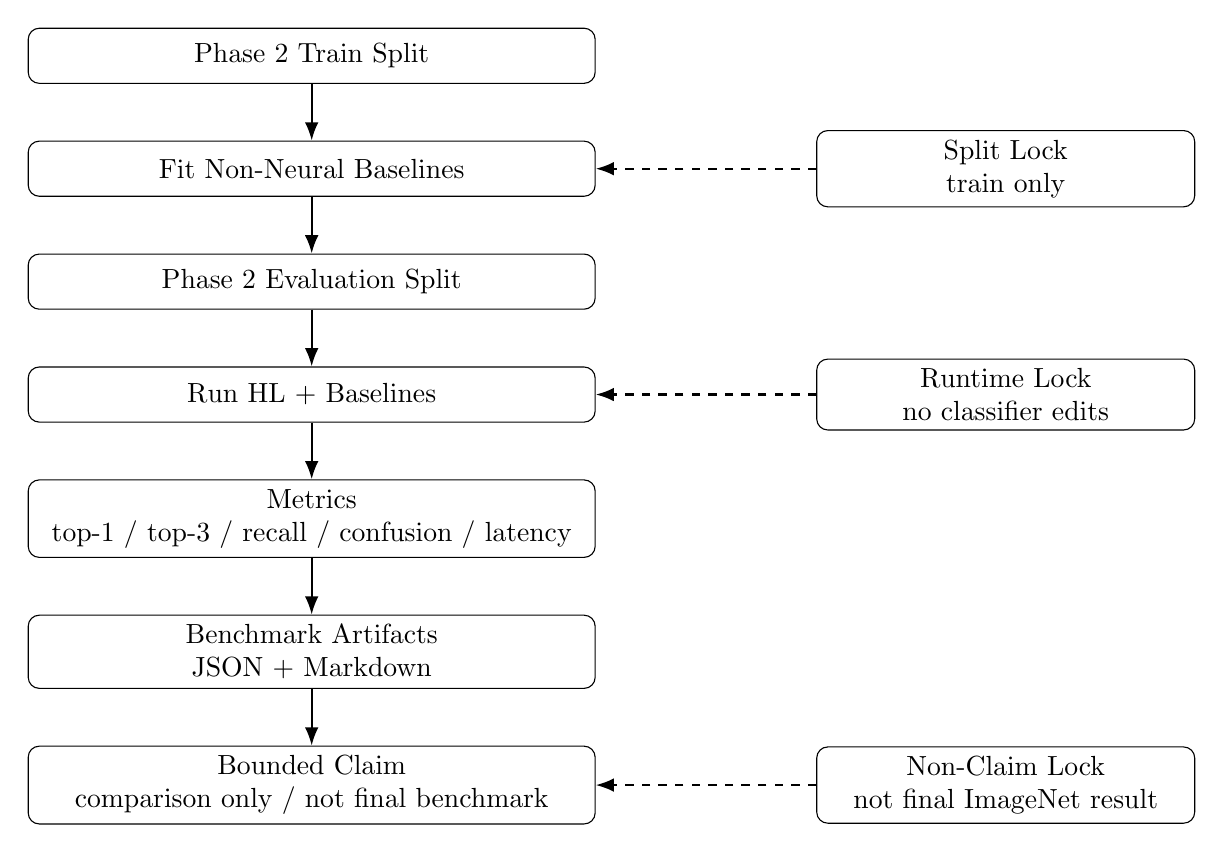
\begin{tikzpicture}[
  node distance=0.72cm,
  box/.style={rectangle, rounded corners, draw, align=center, minimum width=7.2cm, minimum height=0.70cm},
  smallbox/.style={rectangle, rounded corners, draw, align=center, minimum width=4.8cm, minimum height=0.62cm},
  arrow/.style={-Latex, thick}
]

\node[box] (train) {Phase 2 Train Split};
\node[box, below=of train] (fit) {Fit Non-Neural Baselines};
\node[box, below=of fit] (eval) {Phase 2 Evaluation Split};
\node[box, below=of eval] (run) {Run HL + Baselines};
\node[box, below=of run] (metrics) {Metrics\\top-1 / top-3 / recall / confusion / latency};
\node[box, below=of metrics] (artifact) {Benchmark Artifacts\\JSON + Markdown};
\node[box, below=of artifact] (claim) {Bounded Claim\\comparison only / not final benchmark};

\draw[arrow] (train) -- (fit);
\draw[arrow] (fit) -- (eval);
\draw[arrow] (eval) -- (run);
\draw[arrow] (run) -- (metrics);
\draw[arrow] (metrics) -- (artifact);
\draw[arrow] (artifact) -- (claim);

\node[smallbox, right=2.8cm of fit] (splitlock) {Split Lock\\train only};
\draw[arrow, dashed] (splitlock) -- (fit);

\node[smallbox, right=2.8cm of run] (runtime) {Runtime Lock\\no classifier edits};
\draw[arrow, dashed] (runtime) -- (run);

\node[smallbox, right=2.8cm of claim] (nonclaim) {Non-Claim Lock\\not final ImageNet result};
\draw[arrow, dashed] (nonclaim) -- (claim);

\end{tikzpicture}
\end{center}

\section{Validation Surface}

A valid implementation must show:

\begin{enumerate}
\item benchmark architecture exists,
\item baseline module imports,
\item benchmark module imports,
\item runner script executes,
\item train samples load,
\item eval samples load,
\item baselines fit on train,
\item models evaluate on requested split,
\item JSON benchmark emits,
\item Markdown benchmark emits,
\item classifier runtime files remain unchanged.
\end{enumerate}

\[
\boxed{
ValidBench
\Longleftrightarrow
Docs
\wedge
Baselines
\wedge
Run
\wedge
SameSplit
\wedge
Artifacts
\wedge
Locks
\wedge
\neg RuntimeChange.
}
\]

\section{Falsification Surface}

HL-BENCH v1.0 is invalid if:

\begin{itemize}
\item classifier behavior changes,
\item validation is treated as test,
\item baselines train on validation or test,
\item benchmark artifacts are not emitted,
\item model comparison omits split labels,
\item benchmark tooling is presented as classifier improvement,
\item or upstream classifier authorship is blurred.
\end{itemize}

\section{Concluding Compression}

\[
\boxed{
\text{Diagnostics show where Phase 2 fails. Benchmarks show what it beats.}
}
\]

\[
\boxed{
\text{No baseline comparison, no serious performance claim.}
}
\]

\[
\boxed{
\text{Compare first. Tune later. Preserve attribution always.}
}
\]

\end{document}